\documentclass[11pt,a4paper]{article}
\usepackage{isabelle,isabellesym}
\usepackage{fullpage}
\usepackage[usenames,dvipsnames]{color}
\usepackage{graphicx}
\usepackage{document}
%\usepackage[color,cntbysection]{circus}

\usepackage{utp}
\usepackage{pdfpages}

% further packages required for unusual symbols (see also
% isabellesym.sty), use only when needed

\usepackage{amssymb}
  %for \<leadsto>, \<box>, \<diamond>, \<sqsupset>, \<mho>, \<Join>,
  %\<lhd>, \<lesssim>, \<greatersim>, \<lessapprox>, \<greaterapprox>,
  %\<triangleq>, \<yen>, \<lozenge>

\usepackage[english]{babel}
  %option greek for \<euro>
  %option english (default language) for \<guillemotleft>, \<guillemotright>

\usepackage[only,bigsqcap]{stmaryrd}
  %for \<Sqinter>

\usepackage{eufrak}
  %for \<AA> ... \<ZZ>, \<aa> ... \<zz> (also included in amssymb)

%\usepackage{textcomp}
  %for \<onequarter>, \<onehalf>, \<threequarters>, \<degree>, \<cent>,
  %\<currency>

\usepackage{stmaryrd}

% this should be the last package used
\usepackage{pdfsetup}

% urls in roman style, theory text in math-similar italics
\urlstyle{rm}
\isabellestyle{it}

% for uniform font size
%\renewcommand{\isastyle}{\isastyleminor}

\newcommand{\dcomp}{;}%

\setcounter{topnumber}{1}
\setcounter{bottomnumber}{1}
\setcounter{totalnumber}{1}

\usepackage{subcaption}
% tikz
\usepackage{tikz}
\usetikzlibrary{shapes,arrows,trees,positioning,shadows}
\usetikzlibrary{fit}					% fitting shapes to coordinates
\usetikzlibrary{backgrounds}	        % drawing the background after the foreground
\usetikzlibrary{calc}	                % for coordination calculation 
\usetikzlibrary{fadings}                % fading shadow
\usetikzlibrary{decorations.text}
\usetikzlibrary[intersections]			% name path

\pgfdeclarelayer{bg}    % declare background layer
\pgfdeclarelayer{fg}    % declare background layer
\pgfsetlayers{bg,main,fg}  % set the order of the layers (main is the standard layer)

\tikzset{
block/.style = {draw, fill=white, rectangle, minimum height=3em, minimum width=3em},
tmp/.style  = {coordinate}, 
sum/.style= {draw, fill=white, circle, node distance=1cm},
input/.style = {coordinate},
output/.style= {coordinate},
pinstyle/.style = {pin edge={to-,thin,black}
}
}

\begin{document}

\title{Compositional Assume-Guarantee Reasoning of Control Law Diagrams using UTP}

\author{Kangfeng Ye \and Simon Foster \and Jim Woodcock \\[.5ex] University of York, UK \\[2ex] \texttt{\small $\{$kangfeng.ye,simon.foster,jim.woodcock$\}$@york.ac.uk}}

\maketitle

\begin{abstract}
    This report is a summary of our work for the VeTSS funded project ``Mechanised Assume-Guarantee Reasoning for Control Law Diagrams via Circus''. Our Assume-Guarantee (AG) reasoning of control law diagrams is based on Hoare and He's Unifying Theories of Programming and their theory of designs. In this report, we present developed theories and laws to map discrete-time Simulink block diagrams to designs in UTP, calculate assumptions and guarantees, and verify properties for modelled systems. A practical application of our AG reasoning to an aircraft cabin pressure control subsystem is also presented. In addition, all mechanised theories in Isabelle/UTP are attached in Appendices. In the end of this report, we summarise current progress for each work package.
\end{abstract}

\tableofcontents

% sane default for proof documents
\parindent 0pt\parskip 0.5ex

\section{Introduction} \label{sec:intro}
Control law diagrams such as Simulink~\cite{Simulink} and OpenModelica~\cite{openmodelica} are widely used industrial languages and tool-sets for expressing control laws, including support for simulation and code generation. In particular, Simulink actually is a \emph{de facto} standard in many areas in industry. Its model based design, simulation and code generation make it a very efficient and cost-effective way to develop complex systems. Though empirical analysis through simulation is an important technique to explore and refine models, only formal verification can make specific mathematical guarantees about behaviour, which is crucial to ensure safety of associated implementations. Whilst verification facilities for Simulink exist~\cite{Arthan2000, Roy2011, Bostroem2016, Caspi2003, Cavalcanti2005a, Preoteasa2017}, there is still a need for assertional reasoning techniques that capture the full range of specifiable behaviour, provide non-deterministic specification constructs, and support compositional verification. Such techniques also need to be sufficiently expressive to handle the plethora of additional languages and modelling notations that are used by industry in concert with Simulink, in order to allow formulation of heterogeneous "multi-models" that capture the different paradigms and disciplines used in large scale systems~\cite{Zeyda2018}. Applicable tool support for these techniques with a high degree of automation is also of vital importance to enable adoption by industry. Since Simulink diagrams are data rich and usually have an uncountably infinite state space, model checking alone is insufficient and there is a need for theorem proving facilities.

Assume-Guarantee (AG) reasoning is a valuable compositional verification technique for reactive systems~\cite{Meyer1992, Jones2003, Bauer2012}. In AG, one demonstrates composite system level properties by decomposing them into a number of contracts for each component subsystem. Each contract specifies the guarantees that the subsystem will make about its behaviour, under certain specified assumptions of the subsystem's environment. Such a decomposition is vital in order to make verification of a complex system tractable, and to allow development of subsystems by separate teams. AG reasoning has previously been applied to verification of discrete time Simulink control law diagrams through mappings into synchronous languages like Lustre~\cite{Tripakis2005} and Kahn Process Networks~\cite{Bostroem2016}. However such formalisms, whilst theoretically and practically appealing, are limited to expressing processes that are inherently deterministic and non-terminating in nature. Refinement Calculus for Reactive Systems (RCRS)~\cite{Preoteasa2017} is a methodology that can be applied to reason about non-deterministic and non-input-receptive systems by treating programs as predicate transformers. However, it is not able to reason about multi-rate Simulink diagrams and algebraic loops. Almost all these verification facilities translate Simulink to sequential languages, synchronous languages or reactive languages~\cite{Cavalcanti2005a}, and then use verification methods for these languages to reason about Simulink diagrams. There is a need to develop a reasoning technique that is based on the semantic understanding of simulation in Simulink as described in Section~\ref{ssec:simulink}. Thus, it is necessary to translate to several additional notations where AG verification can be performed, which hampers both traceability and composition with other languages of different paradigms. What is needed is a rich unified language capable of AG reasoning, and supported by theorem proving, into which Simulink and associated notations can be losslessly translated.

Our proposed approach thus explores development of formal AG-based proof support for discrete-time Simulink diagrams through a semantic embedding of the theory of designs~\cite{Woodcock2004} in Unifying Theories of Programming (UTP)~\cite{Hoare1998} in Isabelle/HOL~\cite{Nipkow2002} using our developed tool Isabelle/UTP~\cite{Foster2014}. Initially, we proposed to use \Circus~\cite{Oliveira2009}, a formal modelling language for concurrent and reactive systems in the style of CSP, to model Simulink diagrams as shown in~\cite{Cavalcanti2005a}, and then apply contract-based reasoning to \Circus. A \Circus\ model consists of a network of processes that communicate with one another solely via shared channels that carry typed data. Internal state variables are encapsulated and not directly observable by other parallel processes. \Circus\ can capture a variety of languages at the semantic level, and thus supports the formulation of heterogeneous multi-models~\cite{Zeyda2018} by acting as a ``lingua franca''. In addition, a timed version of \Circus\ is used to model multi-rate diagrams. However, a \Circus\ model has more complex information of blocks in Simulink for AG reasoning. For example, the corresponding \Circus\ process for a block uses channels to model connections in diagrams, a non-deterministic internal choice of all input channels to allow an arbitrary input order, and similarly an internal choice of output channels to allow an arbitrary output order. 

In order to reason about the \Circus\ model, we need to take trace information into account and traces inevitably are more complicated if there are many inputs and outputs for a block. Eventually, using model checking or theorem proving to verify \Circus\ models becomes more difficult. According to the semantic understanding of simulation in Simulink in Section~\ref{ssec:simulink}, actually the order of inputs and outputs is irrelevant. Therefore, we have changed our approach to use the theory of designs in UTP to enable AG reasoning for Simulink block diagrams. 

A \emph{design} in UTP is a relation between two predicates where the first predicate (precondition) records the assumption and the second one (postcondition) specifies the commitment. \emph{Designs} are intrinsically suitable for modelling and reasoning about state-based programs (such as B machines~\cite{Abrial2005} and Z notations~\cite{Spivey1989}) but not necessary for reactive programs. For simulation of Simulink diagrams, we discretise the simulation time and abstract it into steps (natural numbers), and define inputs and outputs of Simulink blocks as a function from step numbers to a list of inputs or outputs. In this way, the reactive behaviour is encoded in the step numbers in functions. Finally, the theory of designs can be used to reason about reactive behaviour of Simulink diagrams without introduction of detailed implementation information .

Our work presented in this report has multiple contributions. The main contribution is to define a theoretical reasoning framework for control law block diagrams using the theory of designs in UTP. Each block or subsystem is translated to a design and then hierarchical connections of blocks are mapped to a variety of compositions of designs. Additionally, the refinement relation of designs, monotony of composition operators, and closure laws enable compositional reasoning of block diagrams using a contract-based methodology. The second contribution is our mechanisation of theories in the theorem prover Isabelle using our implementation of UTP, Isabelle/UTP. Then the practical contribution is our industrial case study of a subsystem in a safety critical aircraft cabin pressure control system.

In the next section, we describe the relevant preliminary background about Simulink and UTP. Then in Section~\ref{sec:assum}, the assumptions we made are presented and a brief reasoning procedure is described. Section~\ref{sec:trans} defines our treatment of blocks in UTP and translations of a number of blocks are illustrated. Furthermore, we introduce our composition operators and their corresponding theorems in Section~\ref{sec:comp}. Afterwards, in Section~\ref{sec:case} we briefly describe the industrial case study. And we conclude our work in Section~\ref{sec:conclu}. Additionally, our mechanised theories, laws and case studies are attached in appendices.


\section{Preliminaries}\label{sec:prel}
\subsection{Control Law Diagrams and Simulink} \label{ssec:simulink}
Simulink is a model-based design modelling, analysis and simulation tool for signal processing systems and control systems. It offers a graphical modelling language which is based on hierarchical block diagrams. Its diagrams are composed of subsystems and blocks as well as connections between these subsystems and blocks. In addition, subsystems also can consists of others subsystems and blocks. And single function blocks have inputs and outputs, and some blocks also have internal states.

There is no formal semantics for Simulink. A consistent understanding \cite{Marian2007, Cavalcanti2013} of the simulation in Simulink is based on an \emph{idealized} time model. All executions and updates of blocks are performed \emph{instantaneously} (and infinitely fast) at exact simulation steps. Between the simulation steps, the system is \emph{quiescent} and all values held on lines and blocks are constant. The inputs, states and outputs of a block can only be updated when there is a time hit for this block. Otherwise, all values held in the block are constant too though at exact simulation steps. According to this idealized time model, it is inappropriate to assume that blocks are sequentially executed. For example, for a block it is inappropriate to say it takes its inputs, calculates its outputs and states, and then outputs the results from this point of view. Simulation and code generation of Simulink diagrams use sequential semantics for implementation. But it is not always necessary. 
Simulink needs to have a mathematical and denotational semantics, which UTP provides.

Based on the idealized time model, a single function block can be regarded as a relation between its inputs and outputs. For instance, a unit delay block specifies that its initial output is equal to its initial condition and its subsequent output is equal to previous input. Then connections of blocks establish further relations between blocks. A directed connection from one block to another block specifies that the output of one block is equal to the input of another block. Finally, hierarchical block diagrams establish a relation network between blocks and subsystems. 

\subsection{Unifying Theories of Programming}
UTP is a unified framework to provide a theoretical basis for describing and specifying computer languages across different paradigms such as imperative, functional, declarative, nondeterministic, concurrent, reactive and high-order. A theory in UTP is described using three parts: %\emph{alphabet}, \emph{signature} and \emph{healthiness conditions}. 
\emph{alphabet}, a set of variable names for the theory to be studied; \emph{signature}, rules of primitive statements of the theory and how to combine them together to get more complex program; and \emph{healthiness conditions}, a set of mathematically provable laws or equations to characterise the theory.

The alphabetised relational calculus \cite{Cavalcanti2004} is the most basic theory in UTP. A relation is defined as a predicate with undecorated variables ($v$) and decorated variables ($v'$) in its alphabet. $v$ denotes the observation made initially and $v'$ denotes the observation made at the intermediate or final state. 

The understanding of the simulation in Simulink is very similar to the concept ``programs-as-predicates''~\cite{Hoare1984}. This is the similar idea that the Refinement Calculus of Reactive Systems (RCRS) \cite{Preoteasa2017} uses to reason about reactive systems. RCRS is a compositional formal reasoning framework for reactive systems. The language is based on monotonic property transformers which is an extension of monotonic predicate transformers~\cite{Preoteasa2014b}.  This semantic understanding makes Unifying Theories of Programming (UTP) \cite{Hoare1998} intrinsically suitable for reasoning of the semantics of Simulink simulation because UTP uses an alphabetised predicate calculus to model computations.

Refinement calculus is an important concept in UTP. Program correctness is denoted by $S \refinedby P$, which means that the observations of the program $P$ must be a subset of the observations permitted by the specification $S$. For instance, $(x = 2)$ is a refinement of the predicate $(x > 1)$. A refinement sequence is shown in (\ref{refine_seq}). $S1$ is more general and abstract specification than $S2$ and thus more easier to implement. The predicate $\ptrue$ is the easiest one and can be implemented by anything. $P2$ is more specific and determinate program than $P1$ and thus $P2$ is more useful in general. $\pfalse$ is the strongest predicate and it is impossible to implement in practice.
%{\setlength{\abovedisplayskip}{1pt}
\begin{flalign}
		\textbf{true} \refinedby S1 \refinedby S2 \refinedby P1 \refinedby P2 \refinedby \textbf{false} \label{refine_seq}
\end{flalign}
%%

\subsubsection{Designs}
\emph{Designs} are a subset of the alphabetised predicates that use a particular variable $ok$ to record information about the start and termination of programs. The behaviour of a design is described from initial observation and final observation by relating its precondition $P$ (assumption) to the postcondition $Q$ (commitment) as $\design{P}{Q}$ \cite{Woodcock2004, Hoare1998} (assuming $P$ holds initially, then Q is established). Therefore, the theory of designs is intrinsically suitable for assume-guarantee reasoning~\cite{Foster2017b}. 

\begin{definition}[Design] \label{def:design} 
  \begin{align*}
      & \design{P}{Q} \defs P \land ok \implies Q \land ok' & 
  \end{align*}
\end{definition}
A design is defined in \ref{def:design} where $ok$ records the program has started and $ok'$ that it has terminated. It states that if the design has started ($ok=\logtrue{}$) in a state satisfying its precondition $P$, then it will terminate ($ok'=\logtrue{}$) with its postcondition $Q$ established. We introduce some basic designs.

\begin{definition}[Basic Designs] \label{def:basic_des}
  \begin{align*}
      \topD ~~\defs~~& \design{\true}{\false} = \lnot ok \tag*{[Miracle]}\\
      \botD ~~\defs~~& \design{\false}{\false} = \trueD \tag*{[Abort]}\\
      (x := e) ~~\defs~~& \left(\design{\true}{x'=e\land y' = y \land \cdots}\right) \tag*{[Assignment]} \\ 
      \IID ~~\defs~~& \left(\design{\true}{\II}\right) \tag*{[Skip]}
  \end{align*}
\end{definition}

Abort ($\botD$) and miracle ($\topD$) are the top and bottom element of a complete lattice formed from designs under the refinement ordering. Abort ($\botD$) is never guaranteed to terminate and miracle establishes the impossible. In addition, abort is refined by any other design and miracle refines any other designs. Assignment has precondition $\true$ provided the expression $e$ is well-defined and establishes that only the variable $x$ is changed to the value of $e$ and other variables have not changed. The skip $\IID$ is a design identity that always terminates and leaves all variables unchanged.

Designs can be sequentially composed with the following theorem:
\begin{theorem}[Sequential Composition] \label{thm:des_seq}
    \begin{align*}
    %    \left(\design{P_1}{Q_1} \relsemi \design{P_2}{Q_2}\right) ~~=~~& 
    %        \left(\design{\left(\lnot\left(\lnot P_1 \relsemi \true\right) \land \lnot \left(Q_1 \relsemi \lnot P_2\right)\right)}{Q_1 \relsemi Q_2}\right)\\
    %                                                              ~~=~~& 
    %        \left(\design{\left(\lnot\left(\lnot P_1 \relsemi \true\right) \land \left(Q_1 \mywp P_2\right)\right)}{Q_1 \relsemi Q_2}\right)\\
        \left(\design{p_1}{Q_1} \relsemi \design{P_2}{Q_2}\right) ~~=~~& 
        \left(\design{\left(p_1 \land \lnot \left(Q_1 \relsemi \lnot P_2\right)\right)}{Q_1 \relsemi Q_2}\right) \tag*{[$p_1$-condition]}
    \end{align*}
\end{theorem}

A sequence of designs terminates when $p_1$ holds and $Q_1$ guarantees to establish $P_2$ provided $p_1$ is a condition. On termination, sequential composition of their postconditions is established. A condition is a particular predicate that only has input variables in its alphabet. In other words, a design of which its precondition is a condition only makes the assumption about its initial observation (input variables) and without output variables. That is the same case for our treatment of Simulink blocks. Furthermore, sequential composition has two important properties: associativity and monotonicity which are given in the theorem below.
\begin{theorem}[Associativity, Monotonicity]
    \begin{align*}
        & P_1 \dcomp \left(P_2 \dcomp P_3\right) = \left(P_1 \dcomp P_2\right) \dcomp P_3 & \tag*{[Associativity]} \\
        & \left(P_1 \dcomp Q_1\right) \refinedby \left(P_2 \dcomp Q_2\right) & \tag*{[Monotonicity]} 
    \end{align*}
    \label{thm:seq}
\end{theorem}

Refinement of designs is given in the theorem below.
\begin{theorem}[Refinement]
    \begin{align*}
        \left(\design{P_1}{Q_1} \refinedby \design{P_2}{Q_2}\right) ~~=~~& \left(P_2 \refinedby P_1\right) \land \left(Q_1 \refinedby P_1 \land Q_2\right)\\
                                                     ~~=~~& \left[P_1 \implies P_2\right] \land \left[P_1 \land Q_2 \implies Q_1\right]\\
    \end{align*}
\end{theorem}
Refinement of designs is achieved by either weakening the precondition, or strengthening the postcondition in the presence of the precondition.

In addition, we define two notations $pre_D$ and $post_D$ to retrieve the precondition of the design and the postcondition in the presence of the precondition. 
\begin{definition}[$pre_D$ and $post_D$]
    \begin{align*}
        & pre_D\left(\design{P}{Q}\right) \defs P & \\
        & post_D\left(\design{P}{Q}\right) \defs \left(P \implies Q\right) & \\
    \end{align*}
\end{definition}



\section{Assumptions and General Procedure of Reasoning}
\label{sec:assum}
\subsection{Assumptions}
\emph{Causality} We assume the discrete-time systems modelled in Simulink diagrams are \emph{causal} where the output at any time only depends on values of present and past inputs. Consequently, if inputs to a casual system are identical up to some time, their corresponding outputs must also be equal up to this time.

\emph{Single-rate} This mechanised work captures only single sampling rate Simulink models, which means the timestamps of all simulation steps are multiples of a base period $T$. Eventually, steps are abstracted and measured by step numbers (natural numbers $\nat$) and $T$ is removed from its timestamp. 

An \emph{algebraic loop} occurs in simulation when there exists a signal loop with only direct feedthrough blocks in the loop, such as instantaneous feedback without delay in the loop. \cite{Bostroem2016, Caspi2003, Dragomir2016} assume there are no algebraic loops in Simulink diagrams and RCRS~\cite{Preoteasa2017} identifies it as a future work. Our theoretical framework can reason about discrete-time block diagrams with algebraic loops: specifically check if there are solutions and find the solutions.

The signals in Simulink can have many data types, such as signed or unsigned integer, single float, double float, and boolean. %nine basic types, enumeration, complex, vector and matrix, fixed data type, and bus object. 
The default type for signals are \emph{double} in Simulink. This work uses real numbers in Isabelle/HOL as a universal type for all signals. Real numbers in Isabelle/HOL are modelled precisely using Cauchy sequences, which enables us to reason in the theorem prover. This is a reasonable simplification because all other types could be expressed using real numbers, such as boolean as 0 and 1. 

%Signal as a function from simulation time to a universal real type, model scalar now but could be extended to support vector and matrix
%
%Normal design (precondition is a condition): all outputs could be expressed as relation to inputs only, therefore even outputs are referred in preconditions but they are able to be converted into equal expressions with inputs only.
%
%Deterministic (if there is a solution for a feedback diagram, it must be unique.)
%
%Non-terminating
%
%Fixed number of inputs and outputs: SimBlock condition

\subsection{General Procedure of Applying Assumption-Guarantee Reasoning}
Simulink blocks are semantically mapped to designs in UTP where additionally we model assumptions of blocks to avoid unpredictable behaviour (such as a divide by zero error in the Divide block) and ensure healthiness of blocks. The general procedure of applying AG reasoning to Simulink blocks is given below.

\begin{itemize}
    \item Single blocks and atomic subsystems are translated to single designs with assumptions and guarantees, as well as block parameters. This is shown in Section~\ref{sec:trans}.
    \item Hierarchical block connections are modelled as compositions of designs ($I$) by means of sequential composition, parallel composition and feedback.
    \item Properties or Requirements of block diagrams ($S$) to be verified are modelled as designs as well.
    \item The refinement relation ($S \refinedby I$) in UTP is used to verify if a given property is satisfied by a block diagram (or a subsystem) or not. Our approach supports compositional reasoning according to monotonicity of composition operators in terms of the refinement relation. Provided two properties $S_1$ and $S_2$ are verified to hold in two blocks or subsystems $I_1$ and $I_2$ respectively, then composition of the properties is satisfied by the composition of the blocks or subsystems in terms of the same operator.
   \begin{align*}
      & \left(S_1 \refinedby I_1 \land  S_2 \refinedby I_2\right) \implies \left(S_1 \ op\ S_2 \refinedby I_1 \ op\ I_2\right) &
   \end{align*}
\end{itemize}


\section{Semantic Translation of Blocks}
\label{sec:trans}

In this section, we focus on the methodology to map individual Simulink blocks to designs in UTP semantically. Basically, a block or subsystem is regarded as a relation between inputs and outputs. We use an undashed variable and a dashed variable to denotes input signals and output signals respectively.

\subsection{State Space}
The state space of our theory for block diagrams is composed of only one variable in addition to $ok$, named $inouts$. Originally, we defined it as a function from real numbers (time $t$) to a list of inputs or outputs. Each element in the list denotes an input or output and their order in the list is the order of input or output signals.
\begin{align*}
    inouts: \real_{\geq 0}\fun \seq \real
\end{align*}

However, according to our single-rate assumption, the timestamp at time $t$ is equal to multiples of a basic period $T$: $inouts(t) = inouts(n*T)$. Then $T$ is abstracted away and only the step number $n$ is related. Finally, it is defined below.

\begin{align*}
    inouts : \nat \fun \seq \real
\end{align*}

Then a block is a design that establishes the relation between an initial observation $inouts$ (a list of input signals) and a final observation $inouts'$ (a list of output signals). Additionally, this is subject to the assumption of the design.

\subsection{Healthiness Condition: $\healthy{SimBlock}$}
This healthiness condition characterises a block with a fixed number of inputs and outputs. Additionally it is feasible. A design is a feasible block if there exists at least a pair of $inouts$ and $inouts'$ that establishes both the precondition and postcondition of the design.

\begin{definition}[$\healthy{SimBlock}$]
    A design $P$ with $m$ inputs and $n$ outputs is a Simulink block if $P$ is $\healthy{SimBlock}$ healthy.
    \begin{align*}
       \healthy{SimBlock}(m, n, P) \defs \left( 
       \begin{array}[]{l}
       \left(pre_D(P) \land post_D(P) \neq \false\right) \land \\
       \left(\left(\forall n @ \#\left(inouts~n\right) = m\right) \refinedby Dom~\left(pre_D(P) \land post_D(P)\right)\right) \\
       \left(\left(\forall n @ \#\left(inouts~n\right) = n\right) \refinedby Ran~\left(pre_D(P) \land post_D(P)\right)\right)
       \end{array}\right)
    \end{align*}
    where $Dom$ and $Ran$ calculate the characteristic predicate for domain and range. Their definitions are shown below.
    \begin{align*}
       &Dom(P) \defs \left(\exists inouts' @ P\right) & \\  
       &Ran(P) \defs \left(\exists inouts @ P\right) &
    \end{align*}
\end{definition}

$inps$ and $outps$ are the operators to get the number of input signals and output signals for a block. They are implied from $\healthy{SimBlock}$ of the block. 
\begin{definition}[$inps$ and $outps$]
\begin{align*}
   \healthy{SimBlock}(m, n, P) \implies \left(inps(P) = m \land outps(P) = n\right) 
\end{align*}
    Provided that $P$ is a healthy block, $inps$ returns the number of its inputs and $outps$ returns the number of its outputs.
\end{definition}

\subsection{Blocks}
In order to give definitions of the corresponding designs for Simulink blocks, firstly we define a design pattern $FBlock$. Then we illustrate definitions of two typical Simulink blocks and three additional virtual blocks using this pattern. The definitions of all other blocks could be found in Appendix~\ref{sec:block_theories}.

\subsubsection{Pattern}
We defined a pattern that is used to define all other blocks.
\begin{definition}[$FBlock$]
\begin{align*}
    & FBlock\left(f_1, m, n, f_2\right) &\\
    &\defs \left(
            \vdesign{\forall nn @ f_1\left(inouts, nn\right)}
                    {\forall nn @ \left(
                        \begin{array}[]{l}
                            \#\left(inouts(nn)\right) = m \land \\
                            \#\left(inouts'(nn)\right) = n \land \\
                            \left(inouts'(nn) = f_2\left(inouts'(nn), nn\right)\right) \land \\ 
                            \left(\forall sigs:\nat \fun \seq~\real, nn:\nat @ \#\left(sigs~nn\right) = m \implies \#\left(f_2(sigs, nn)\right) = n\right)
                        \end{array} \right)
                    }
        \right) &
\end{align*}
\end{definition}

$FBlock$ has four parameters: $f_1$ is a predicate that specifies the assumption of the block and it is a function on input signals; $m$ and $n$ are the number of inputs and outputs, and $f_2$ is a function that relates inputs to outputs and is used to establish the postcondition of the block. The precondition of $FBlock$ states that $f_1$ holds for inputs at any step $nn$. And the postcondition specifies that for any step $nn$ the block always has $m$ inputs and $n$ outputs, the relation between outputs and inputs are given by $f_2$, and additionally $f_2$ always produces $n$ outputs provided there are $m$ inputs.

\subsubsection{Simulink Blocks}
\begin{definition}[Unit Delay] \label{def:ud}
    \begin{align*}
        UnitDelay\left(x_0\right) \defs FBlock\left( \logtrue{f}, 1, 1, \left(\lambda x, n @ \langle \condition{x_0}{n = 0}{hd\left(x~(n-1)\right)}\rangle\right)\right) 
    \end{align*}
    where $hd$ is an operator to get the head of a sequence, and $\logtrue{f} = \left(\lambda x, n @ \logtrue{}\right)$ that means no constraints on input signals.
\end{definition}
The definition \ref{def:ud} of the Unit Delay block is straightforward: it accepts all inputs, has one input and one output, and produces initial value $x_0$ in its first step (0) and the previous input otherwise.

\begin{definition}[Product (Divide)] \label{def:div2}
    \begin{align*}
        Div2 \defs FBlock\left( \left(\lambda x, n @ hd(tl(x~n)) \neq 0\right), 2, 1, \left(\lambda x, n @ \langle hd(x~n)/hd(tl(x~n))\rangle\right)\right) 
    \end{align*}
    where $tl$ is an operator to get the tail of a sequence.
\end{definition}
The definition \ref{def:div2} of Divide block is slightly different because it assumes the input value of its second input signal is not zero at any step. By this way, the precondition enables modelling of non-input-receptive systems that may reject some inputs at some points. %That is the similar case for the square root function in the math block.

\subsubsection{Virtual Blocks}
In addition to Simulink blocks, we have introduced three blocks for the purpose of composition: $Id$, $Split2$, and $Router$. The usage of these blocks is illustrated in Figure~\ref{fig:compose}.

\begin{definition}[Id] \label{def:id}
    \begin{align*}
        Id \defs FBlock\left( \logtrue{f}, 1, 1, \left(\lambda x, n @ \langle hd\left(x~n\right)\rangle\right)\right) 
    \end{align*}
\end{definition}
The identity block $Id$ is a block that has one input and one output, and the output value is always equal to the input value. It establishes a fact that a direct signal line in Simulink could be treated as sequential composition of many $Id$ blocks. The usage of $Id$ is shown in Figure~\ref{fig:id}.

\begin{definition}[Split2]  \label{def:split2}
    \begin{align*}
        Split2 \defs FBlock\left( \logtrue{f}, 1, 2, \left(\lambda x, n @ \langle hd\left(x~n\right), hd\left(x~n\right)\rangle\right)\right) 
    \end{align*}
\end{definition}
$Split2$ corresponds to the signal connection splitter that produces two signals from one and both signals are equal to the input signal. The usage of $Split2$ is shown in Figure~\ref{fig:split}.

\begin{definition}[Router] \label{def:router} 
    \begin{align*}
        Router\left(m, table\right) \defs FBlock\left( \logtrue{f}, m, m, \left(\lambda x, n @ reorder\left(\left(x~n\right), table\right)\right)\right) 
    \end{align*}
\end{definition}
$Router$ corresponds to the crossing connection of signals and this virtual block changes the order of input and output signals according to the supplied table. The usage of $Router$ is shown in Figure~\ref{fig:router}.

\subsection{Subsystems}
The treatment of subsystems (no matter whether hierarchical subsystems or atomic subsystems) in our designs is similar to that of blocks. They could be regarded as a bigger black box that relates inputs to outputs.

\section{Block Compositions}
\label{sec:comp}

In this section, we define three composition operators that are used to compose subsystems or systems from blocks. We also use three virtual blocks to map Simulink's connections in our designs.

For all definitions and laws in this section, if there are no special notes, we assume the following predicates. 
\begin{align*}
    & \healthy{SimBlock}\left(m_1, n_1, P_1\right) & \\
    & \healthy{SimBlock}\left(m_2, n_2, P_2\right) & \\
    & \healthy{SimBlock}\left(m_3, n_3, P_3\right) & \\
    & \healthy{SimBlock}\left(m_1, n_1, Q_1\right) & \\
    & \healthy{SimBlock}\left(m_2, n_2, Q_2\right) & \\
    & P_1 \refinedby Q_1 & \\
    &P_2 \refinedby Q_2 &
\end{align*}

\begin{figure}[htb!]
    \captionsetup[subfigure]{justification=centering}
    \centering 
    \begin{subfigure}[t]{0.3\textwidth}
        \centering 
        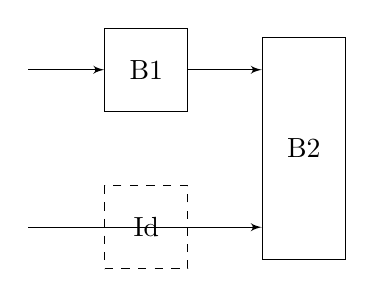
\begin{tikzpicture}[auto, node distance=2cm,>=latex']
            \node [input, name=input1] (input1) {};
            \node [block, right of=input1, node distance=1.5cm] (b1) {B1};
            \node [block, below of=b1, dashed] (id) {Id};
            \node [input, left of=id, node distance=1.5cm] (input2) {};
            \node [block, minimum height=8em] (b2) at ([xshift=2cm, yshift=-1cm]b1){B2};
            \draw [->] (input1) -- (b1);
            \draw [->] (b1) -- (b1 -| b2.west);
            \draw [->] (input2) -- (input2 -| b2.west);
        \end{tikzpicture}
        \caption{Id}
        \label{fig:id}
    \end{subfigure}
    \begin{subfigure}[t]{0.3\textwidth}
        \centering 
        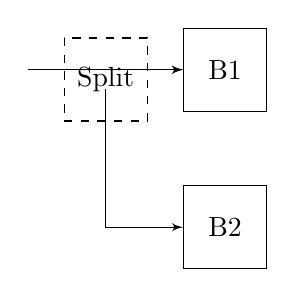
\begin{tikzpicture}[auto, node distance=2cm,>=latex']
            \node [input, name=input1] (input1) {};
            \node [block, right of=input1, node distance=2.5cm] (b1) {B1};
            \node [block, below of=b1] (b2) {B2};
            \draw [->] (input1) --node[name=z,anchor=north]{} (b1);
            \node [block, dashed] (split) at (z) {Split};
            \draw [->] (input1) -- (b1);
            \draw [->] (z) |- (b2);
        \end{tikzpicture}
        \caption{Split}
        \label{fig:split}
    \end{subfigure}
    \begin{subfigure}[t]{0.3\textwidth}
        \centering 
        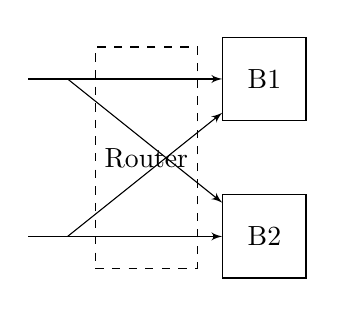
\begin{tikzpicture}[auto, node distance=2cm,>=latex']
            \begin{pgfonlayer}{fg}
                \node [input, name=input1] (input1) {};
                \node [block, right of=input1, node distance=3cm] (b1) {B1};
                \node [block, below of=b1] (b2) {B2};
                \node [input, left of=b2, node distance=3cm] (input2) {};
                \node [block, dashed, minimum height=8em] (router) at ([xshift=1.5cm, yshift=-1cm]input1.east) {Router};
                %\node [output, right of=b1, node distance=1.5cm] (output1) {};
                %\node [output, right of=b2, node distance=1.5cm] (output2) {};
                \draw [->] (input1) --node[name=z1]{} (b1);
                \draw [->] ([xshift=0.5cm]input1) -- (b2);
                %\draw [->] (z1) -- (b2);
                \draw [->] (input2) --node[name=z2]{} (b2);
                \draw [->] ([xshift=0.5cm]input2) -- (b1);
                %\draw [->] (z2) -- (b1);
                %\draw [->] (z1 |- b2.west) -- (z1 -| b2.west);
                %\draw [->] (z2 |- b1.west) -- (z2 -| b1.west);
                %\draw [->] (b2) -- (output2);
            \end{pgfonlayer}
            \begin{pgfonlayer}{bg}
                \node [rectangle, dashed, fit= (b1) (b2), label=left:] {};
            \end{pgfonlayer}
        \end{tikzpicture}
        \caption{Router}
        \label{fig:router}
    \end{subfigure}
    \begin{subfigure}[t]{0.3\textwidth}
        \centering 
        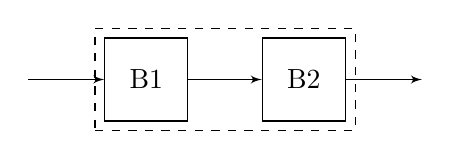
\begin{tikzpicture}[auto, node distance=2cm,>=latex']
            \begin{pgfonlayer}{fg}
                \node [input, name=input1] (input1) {};
                \node [block, right of=input1, node distance=1.5cm] (b1) {B1};
                \node [block, right of=b1] (b2) {B2};
                \node [output, right of=b2, node distance=1.5cm] (output) {};
                \draw [->] (input1) -- (b1);
                \draw [->] (b1) -- (b2);
                \draw [->] (b2) -- (output);
            \end{pgfonlayer}
            \begin{pgfonlayer}{bg}
                \node [rectangle, draw, dashed, fit= (b1) (b2), label=left:] {};
            \end{pgfonlayer}
        \end{tikzpicture}
        \caption{Sequential Composition}
        \label{fig:seq_comp}
    \end{subfigure}
    \begin{subfigure}[t]{0.3\textwidth}
        \centering 
        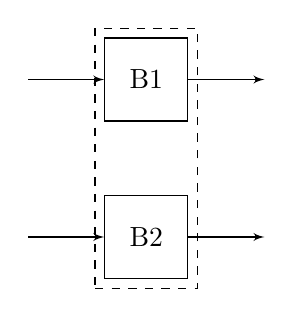
\begin{tikzpicture}[auto, node distance=2cm,>=latex']
            \begin{pgfonlayer}{fg}
                \node [input, name=input1] (input1) {};
                \node [block, right of=input1, node distance=1.5cm] (b1) {B1};
                \node [block, below of=b1] (b2) {B2};
                \node [input, left of=b2, node distance=1.5cm] (input2) {};
                \node [output, right of=b1, node distance=1.5cm] (output1) {};
                \node [output, right of=b2, node distance=1.5cm] (output2) {};
                \draw [->] (input1) -- (b1);
                \draw [->] (b1) -- (output1);
                \draw [->] (input2) -- (b2);
                \draw [->] (b2) -- (output2);
            \end{pgfonlayer}
            \begin{pgfonlayer}{bg}
                \node [rectangle, draw, dashed, fit= (b1) (b2), label=left:] {};
            \end{pgfonlayer}
        \end{tikzpicture}
        \caption{Parallel Composition}
        \label{fig:par_comp}
    \end{subfigure}
    \begin{subfigure}[t]{0.3\textwidth}
        \centering 
        \begin{tikzpicture}[auto, node distance=2cm,>=latex']
            \node [input, name=input1] (input1) {};
            \node [input, below of=input1] (input2) {};
            \node [block, minimum height=6em] (b1) at ([xshift=2cm, yshift=-1cm]input1){B};
            \node [tmp, above of=b1] (tmp1){};
            \node [output, right of=input1, node distance=4cm] (output1) {};
            \node [output, right of=input2, node distance=4cm] (output2) {};
            %\draw [->] (input1) -- (input1 -| b1.west);
            %\draw [->] (input2) -- (input2 -| b1.west);
            %\draw [->] (b1.east) |- (output1) |- (temp1) -| (input1) -- (input1 -| b1.west);
            \draw [->] ([yshift=0.5cm]b1.east) -- ++(0.7cm, 0) -- ++(0,1.1cm) -- ++(-2.6cm, 0) -- ++(0,-1.1cm) -- ([yshift=0.5cm]b1.west);
            \draw [->] ([yshift=-0.5cm]b1.east) -- ++(1cm,0); 
            \draw [->] ([xshift=-1cm, yshift=-0.5cm]b1.west) -- ([yshift=-0.5cm]b1.west); 
        \end{tikzpicture}
        \caption{Feedback}
        \label{fig:fd_comp}
    \end{subfigure}
    \caption{Composition of Blocks}\label{fig:compose}
\end{figure}


\subsection{Sequential Composition}
The meaning of sequential composition of designs is defined in Theorem~\ref{thm:des_seq}. It corresponds to composition of two blocks in Figure~\ref{fig:seq_comp} where the outputs of $B_1$ are equal to the inputs of $B_2$.

Provided 
   \begin{align*}
       \begin{array}[]{ll}
           P = \left(FBlock\left( \logtrue{f}, m_1, n_1, f_1\right)\right) & \qquad \healthy{SimBlock}\left(m_1, n_1, P\right) \\ 
           Q = \left(FBlock\left( \logtrue{f}, n_1, n_2, f_2\right)\right) & \qquad \healthy{SimBlock}\left(n_1, n_2, Q\right) \\ 
       \end{array}
   \end{align*}

The expansion law of sequential composition is given below.
\begin{theorem}[Expansion]
   \begin{align*}
       &\left(P \dcomp Q \right) = FBlock\left( \logtrue{f}, m_1, n_2, (f_2 \circ f_1)\right) & \tag*{[Expansion]}
   \end{align*}
    \label{thm:seq_exp}
\end{theorem}
This theorem establishs that sequential composition of two blocks, where the number of outputs of the first block is equal to the number of inputs of the second block, is simply a new block with the same number of inputs as the first block $P$ and the same number of outputs as the second block $Q$, and additionally the postcondition of this composed block is function composition. In addition, the composed block is still $\healthy{SimBlock}$ healthy which is shown in the closure theorem below.

\begin{theorem}[Closure]
   \begin{align*}
       &\healthy{SimBlock}\left(m_1, n_2, \left(P \dcomp Q \right)\right) & \tag*{[\healthy{SimBlock} Closure]} 
   \end{align*}
    \label{thm:seq_closure}
\end{theorem}

\subsection{Parallel Composition}
Parallel composition of two blocks is a stack of inputs and outputs from both blocks and is illustrated in Figure~\ref{fig:par_comp}. It is defined below.
\begin{definition}[Parallel Composition] \label{def:parallelB} 
    \begin{align*}
        P \parallel_{B} Q \defs \left(
        \begin{array}[]{l}
            \left(takem (inps(P)+inps(Q))~inps(P) \dcomp P \right) \\
            \parallel_{B_M} \\
            \left(dropm (inps(P)+inps(Q))~inps(P) \dcomp Q \right) 
        \end{array} \right)
    \end{align*}
\end{definition}
where $takem$ and $dropm$ are two blocks to split inputs into two parts and their definitions can be found in Appendix~\ref{sec:block_theories}, and $B_M$ is defined below. 
\begin{definition}[$B_M$] \label{def:mergeB} 
    \begin{align*}
        B_M \defs \left(ok' = 0.ok \land 1.ok\right) \land \left(inouts' = 0.inouts \cat 1.inouts\right) 
    \end{align*}
\end{definition}

The definition of parallel composition~\ref{def:parallelB} for designs is similar to the parallel-by-merge scheme~\cite[Sect.~7.2]{Hoare1998} in UTP. Parallel-by-merge is denoted as $P \parallel_M Q$ where $M$ is a special relation that explains how the output of parallel composition of $P$ and $Q$ should be merged following execution. 

However, parallel-by-merge assumes that the initial observations for both predicates should be the same. But that is not the case for our block composition because the inputs to the first block and that to the second block are different. Therefore, in order to use the parallel by merge, firstly we need to partition the inputs to the composition into two parts: one to the first block and another to the second block. This is illustrated in Figure~\ref{fig:parallel} where we assume that $P$ has $m$ inputs and $i$ outputs, and $Q$ has $n$ inputs and $j$ outputs. Finally, it has the same inputs ($m+n$) and the outputs of $P$ and $Q$ are merged by $B_M$ to get $i+j$ outputs.

\begin{figure}[htb]
    \begin{center}
        \includegraphics[scale=0.45]{parallel}
    \end{center}
    \caption{Parallel Composition of Two Blocks}
    \label{fig:parallel}
\end{figure}

The merge operator $B_M$ states that the parallel composition terminates if both blocks terminate. And on termination, the output of parallel composition is concatenation of the outputs from the first block and the outputs from the second block. $takem$ and $dropm$ are two blocks that have the same inputs and the number of inputs is equal to addition of the number inputs of $P$ and the number inputs of $Q$. $takem$ only takes the first part of inputs as required by $P$, and $dropm$ takes the second part of inputs as required by $Q$.

\begin{theorem}[Associativity, Monotonicity, and $\healthy{SimBlock}$ Closure]
    \begin{align*}
        & P_1 \parallel_B \left(P_2 \parallel_B P_3\right) = \left(P_1 \parallel_B P_2\right) \parallel_B P_3 & \tag*{[Associativity]} \\
        & \left(P_1 \parallel_B Q_1\right) \refinedby \left(P_2 \parallel_B Q_2\right) & \tag*{[Monotonicity]} \\ 
        & \healthy{SimBlock}\left(m1+m2, n1+n2, \left(P_1 \parallel_B P_2\right)\right) & \tag*{[\healthy{SimBlock} Closure]} \\ 
        & inps\left(P_1 \parallel_B P_2\right) = m_1 + m_2 & \tag*{} \\
        & outps\left(P_1 \parallel_B P_2\right) = n_1 + n_2 & \tag*{}
    \end{align*}
    \label{thm:parallelB}
\end{theorem}

Parallel composition is associative, monotonic in terms of the refinement relation, and $\healthy{SimBlock}$ healthy. The inputs and outputs of parallel composition are combination of the inputs and outputs of both blocks.

\begin{theorem}[Parallel Operator Expansion]
   Provided 
   \begin{align*}
       \begin{array}[]{ll}
           P = \left(FBlock\left( \logtrue{f}, m_1, n_1, f_1\right)\right) & \qquad \healthy{SimBlock}\left(m_1, n_1, P\right) \\ 
           Q = \left(FBlock\left( \logtrue{f}, m_2, n_2, f_2\right)\right) & \qquad \healthy{SimBlock}\left(m_2, n_2, Q\right) \\ 
       \end{array}
   \end{align*}
   then, 
   \begin{align*}
       \left(P \parallel_B Q\right) = & FBlock\left(
       \begin{array}[]{l}
            \logtrue{f}, m_1+m_2, n_1+n_2, \\
            \left(\lambda x, n @ 
                \left(
                \begin{array}[]{l}
                    \left(f_1 \circ \left(\lambda x, n @ take\left(m_1, x~n\right)\right)\right) \\
                    \cat \left(f_2 \circ \left(\lambda x, n @ drop\left(m_1, x~n\right)\right)\right) 
                \end{array}\right)\right) \\
       \end{array} \right)  & \tag*{[Expansion]} \\
       &\healthy{SimBlock}\left(m_1+m_2, n_1+n_2, \left(P \parallel_B Q\right)\right) & \tag*{[\healthy{SimBlock} Closure]} 
   \end{align*}
    \label{thm:parallel-exp}
\end{theorem}

Parallel composition of two $FBlock$ defined blocks is expanded to get a new block. Its postcondition is concatenation of the outputs from $P$ and the outputs from $Q$. The outputs from $P$ (or $Q$) are function composition of its block definition function $f_1$ (or $f_2$) with $take$ (or $drop$).

\subsection{Feedback}
The feedback operator loops an output back to an input, which is illustrated in Figure~\ref{fig:fd_comp}. 
\begin{definition}[$f_D$]\label{def:fd}
    \begin{align*}
       P~f_D~(i, o) \defs \left(\exists sig @ \left(PreFD(sig, inps(P), i) \dcomp P \dcomp PostFD(sig, outps(P), o)\right) \right)
    \end{align*}
\end{definition}
where $i$ and $o$ denotes the index number of the output signal and the input signal, which are looped. $PreFD$ denotes a block that adds $sig$ into the $i$th place of the inputs.
\begin{definition}[$PreFD$]
    \begin{align*}
       PreFD(sig, m, idx) \defs FBlock\left( \logtrue{f}, m-1, m, \left(f\_PreFD(sig,idx)\right)\right)
    \end{align*}
    where $f\_PreFD(sig, idx) = \lambda x, n @ \left(take(idx, (x~n)) \cat \langle \left(sig~n\right) \rangle \cat drop (idx, (x~n))\right)$ 
    \label{def:prefd}
\end{definition}
and $PostFD$ denotes a block that removes the $o$th signal from the outputs of $P$ and this signal shall be equal to $sig$.
\begin{definition}[$PostFD$]
    \begin{align*}
       PostFD(sig, n, idx) \defs \left(
            \vdesign{\true}
                    {\forall nn @ \left(
                        \begin{array}[]{l}
                            \#\left(inouts(nn)\right) = n \land \\
                            \#\left(inouts'(nn)\right) = n-1 \land \\
                            \left(inouts'(nn) = \left(f\_PostFD(sig, idx, inouts'(nn), nn\right)\right) \land \\ 
                            sig(nn) = inouts(nn)!idx \\
                        \end{array} \right)
                    }
        \right)
    \end{align*}
    where $f\_PostFD(idx) = \lambda x, n @ \left(take(idx, (x~n)) \cat drop (idx+1, (x~n))\right)$ and $!$ is an operator to get the element in a list by its index.
\end{definition}

The basic idea to construct a feedback operator is to use existential quantification to specify that there exists one signal $sig$ that it is the $i$th input and $o$th output, and their relation is established by the block $P$. This is illustrated in Figure~\ref{fig:feedback} where $m$ and $n$ are the number of inputs and outputs of $P$. $PreFD$ adds a signal into the inputs at $i$ and $P$ takes assembled inputs and produces an output in which the $o$th output is equal to the supplied signal. Finally, the outputs of feedback are the outputs of $P$ without the $o$th output. Therefore, a block with feedback is translated to a sequential composition of $PreFD$, $P$, and $PostFD$.

\begin{figure}[htb]
    \begin{center}
        \includegraphics[scale=0.45]{feedback}
    \end{center}
    \caption{Feedback}
    \label{fig:feedback}
\end{figure}

\begin{theorem}[Monotonicity]
    Provided 
    \begin{align*}
        \begin{array}[]{ll}
        \healthy{SimBlock}\left(m_1, n_1, P_1\right) & \qquad \healthy{SimBlock}\left(m_1, n_1, P_2\right) \\
        P_1 \refinedby P_2 & \qquad i_1 < m_1 \land o_1 < n_1 \\
        \end{array}
    \end{align*}
    then,
    \begin{align*} 
       \left(P_1~f_D~(i_1, o_1)\right) \refinedby \left(P_2~f_D~(i_1, o_1)\right)
    \end{align*}
    \label{thm:fd_mono}
\end{theorem}
The monotonicity law states that if a block is a refinement of another block, then its feedback is also a refinement of the same feedback of another block. 

\begin{theorem}[Expansion]
    Provided 
    \begin{align*}
        \begin{array}[]{ll}
            P = FBlock\left( \logtrue{f}, m, n, f\right) & \qquad \healthy{SimBlock}\left(m, n, P\right) \\
            Solvable\_unique(i, o, m, n, f) & \qquad is\_Solution(i, o, m, n, f, sig) \\
        \end{array}
    \end{align*}
    then,
    \begin{align*} 
       & \left(P~f_D~(i, o)\right) & \\
       & = FBlock\left( \logtrue{f}, m-1, n-1, 
       \left(\lambda x, n @ \left(f\_PostFD(o) \circ f \circ f\_PostFD (sig, x, i)\right)~x~n\right)\right) & \tag*{[Expansion]}\\
      & \healthy{SimBlock}\left(m-1,n-1,\left(P~f_D~(i, o)\right)\right) & \tag*{[\healthy{SimBlock} Closure]}
    \end{align*}
    \label{thm:fd_exp}
\end{theorem}
In the expansion theorem, where 
\begin{definition}[$Solvable\_unique$] \label{def:solvable_unique}
    \begin{align*}
       & Solvable\_unique\left(i, o, m, n, f\right) \defs \\
       & \left(
       \begin{array}[]{l}
          \left(i < m \land o < n\right) \land  \\
            \left(\forall sigs @ \left(
                \begin{array}[]{l}
                    \left(\forall nn @ \#\left(sigs~nn\right) = (m - 1)\right) \implies \\
                    \left(\exists_1 sig@\left(\forall nn @ \left(sig~nn = \left(f \left(\lambda n1@ f\_PreFD\left(sig, i, sigs, n1\right), nn\right)\right)!o\right)\right)\right)
                \end{array} \right)\right)
       \end{array}
       \right)
    \end{align*}
\end{definition}
The $Solvable\_unique$ predicate characterises a condition that the block with feedback has a unique solution that satisfies the constraint of feedback: the corresponding output and input are equal. 

\begin{definition}[$is\_Solution$] \label{def:is_solution}
    \begin{align*}
       & is\_Solution\left(i, o, m, n, f,sig\right) \defs \\
       &\left(
       \begin{array}[]{l}
            \left(\forall sigs @ \left(
                \begin{array}[]{l}
                    \left(\forall nn @ \#\left(sigs~nn\right) = (m - 1)\right) \implies \\
                    \left(\forall nn @ \left(sig~nn = \left(f \left(\lambda n1@ f\_PreFD\left(sig, i, sigs, n1\right), nn\right)\right)!o\right)\right)
                \end{array} \right)\right)
       \end{array}
       \right)
    \end{align*}
\end{definition}
The $is\_Solution$ predicate evaluates a supplied signal to check if it is a solution for the feedback.

The expansion law of feedback assumes the function $f$, that is used to define the block $P$, is solvable in terms of $i$, $o$, $m$ and $n$. In addition, it must have one unique solution $sig$ that resolves the feedback. 

Our approach to model feedback in designs enables reasoning about systems with algebraic loops. If a block defined by $FBlock$ and $Solvable\_unique\left(i, o, m, n, f\right)$ is true, then the feedback composition of this block in terms of $i$ and $o$ is feasible no matter whether there are algebraic loops or not.

\subsection{Composition Examples}
For the compositions in Figure~\ref{fig:compose}, their corresponding maps in our design theory are shown below.
\begin{itemize}
    \item Figure~\ref{fig:id}: $\left(B_1 \parallel_B Id\right) \dcomp B_2$ 
    \item Figure~\ref{fig:split}: $Split2 \dcomp \left(B_1 \parallel_B B_2\right)$ 
    \item Figure~\ref{fig:router}: $\left(Split2 \parallel_B Split2\right) \dcomp Router(4, [0,2,1,3]) \dcomp \left(B_1 \parallel_B B_2\right)$ 
    \item Figure~\ref{fig:seq_comp}: $B_1 \dcomp B_2$ 
    \item Figure~\ref{fig:par_comp}: $B_1 \parallel_B B_2$ 
    \item Figure~\ref{fig:fd_comp}: $B~f_D~(0, 0)$ 
\end{itemize}


\section{Case Study}
\label{sec:case}

This case study, verification of a \textsf{post\_landing\_finalize} subsystem, is taken from an aircraft cabin pressure control application. The original Simulink model is from \href{https://www.honeywell.com/}{Honeywell} through our industrial link with \href{http://www.drisq.com/}{D-RisQ}. This case is also studied in \cite{Bhatt2016} and the diagram shown in Figure~\ref{fig:case} is from the paper. The purpose of this subsystem is to implement that the output $finalize\_event$ is triggered after the aircraft door has been open for a minimum specific amount of time following a successful landing. 

\begin{figure}[htb!]
    \begin{center}
        \includegraphics[scale=0.55]{postlanding}
    \end{center}
    \caption{Post Landing Finalize (source: \cite{Bhatt2016})}
    \label{fig:case}
\end{figure}

In order to apply our AG reasoning into this Simulink model, firstly we model the subsystem in our block theories as shown in Section~\ref{ssec:case_model}. Then we verify a number of properties for three small subsystems in this model, which is given in Section~\ref{ssec:case_veri}. Finally, in Section~\ref{ssec:case_req} we present verification of four requirements of this subsystem. To avoid confusion between the subsystem and three small subsystems, in the following sections we use the \emph{system} to denote the \textsf{post\_landing\_finalize} subsystem to be verified, and the \emph{subsystems} to denote three small subsystems.

\subsection{Modelling}
\label{ssec:case_model}

We start with translation of three small subsystems (\textsf{variableTimer}, \textsf{rise1Shot} and \textsf{latch}) according to our block theories. 

The subsystem \textsf{latch} is modelled as below. It is shown in Appendix~\ref{ssec:plf_latch} as well.
\begin{align*}
   & \left(\left(\left(\left((UnitDelay~0) \parallel_B Id\right) \dcomp (LopOR~2) \right) \parallel_B \left(Id \dcomp LopNOT\right) \right) \dcomp \left(LopAND~2\right) \dcomp Split2 \right)\ f_D\ (0,0) &
\end{align*}
The blocks $LopOR$, $LopNOT$ and $LopAND$ correspond to the OR, NOT and AND operators in the logic operator block. Their definitions can be found in Appendix~\ref{sec:block_theories}.  Then we apply composition definitions, expansion and SimBlock closure laws to simplify the subsystem. The \textsf{latch} subsystem is finally simplified to a design.
\begin{align*}
    & latch = FBlock \left( \logtrue{f}, 2, 1, latch\_simp\_pat\_f\right) &
\end{align*}
where the definition of $latch\_simp\_pat\_f$ is given in Appendix~\ref{sec:post_landing}. 

Similarly, \textsf{variableTimer} and \textsf{rise1Shot} are modelled and simplified as shown in Appendix~\ref{ssec:plf_variableTimer} and~\ref{ssec:plf_rise1Shot} respectively. 

Finally, we can use the similar way to compose the three subsystems with other blocks in this diagram to get the corresponding composition of \textsf{post\_landing\_finalise\_1}, and then apply the similar laws to simplify it further into one block and verify requirements for this system. However, for the outermost feedback it is difficult to use the similar way to simplify it into one block because it is more complicate than feedbacks in other three small subsystems (\textsf{variableTimer}, \textsf{rise1Shot} and \textsf{latch}). In order to use the expansion theorem~\ref{thm:fd_exp} of feedback, we need to find a solution for the block and prove the solution is unique. With increasing complexity of blocks, this expansion is becoming harder and harder. Therefore, \textsf{post\_landing\_finalise\_1} has not been simplified into one block. Instead, it is simplified to a block with a feedback which can be seen in the lemma \emph{post\_landing\_finalize\_1\_simp} in Appendix~\ref{sec:post_landing}.
\begin{align*}
  & post\_landing\_finalize\_1 = plf\_rise1shot\_simp\ f_D\ (4, 1) &
\end{align*}

\subsection{Subsystems Verification}
\label{ssec:case_veri}
After simplification, we can verify properties of the subsystems using the refinement relation. 

We start with verification of a property for \textsf{variableTimer}: \emph{vt\_req\_00}. This property states that if the door is closed, then the output of this subsystem is always false. The verification of this property is given in Appendix~\ref{ssec:plf_vt_veri}. However, this property can not be verified in absence of an assumption made to the second input: \emph{door\_open\_time}. This is due to a type conversion block \texttt{int32} used in the subsystem. If the input to \texttt{int32} is larger than $2147483647$ (that is, \emph{door\_open\_time} larger than $2147483647/10$), its output is less than zero and finally the output is true. That is not the expected result. Practically, \emph{door\_open\_time} should be less than $2147483647/10$. Therefore, we can make an assumption of the input and eventually verify this property as given in the lemma \emph{vt\_req\_00}. Additionally, we suggest a substitution of \texttt{int32} by \texttt{uint32}, or a change of the data type for the input from double to unsigned integer, such as \texttt{uint32}. 

As for the \textsf{rise1Shot} subsystem, we verified one property: \emph{rise1shot\_req\_00}. This property specifies that the output is true only when current input is true and previous input is false (see Appendix~\ref{ssec:plf_rise1shot_veri}). It means it is triggered only by a rising edge and continuous true inputs will not enable the output.

Furthermore, one property for the \textsf{latch} subsystem (a SR AND-OR latch) is verified (see Appendix~\ref{ssec:plf_latch_veri}). The property \emph{latch\_req\_00} states that as long as the second input $R$ is true, its output is always false. This is consistent with the definition of the SR latch in circuits.

\subsection{Requirement Verification}
\label{ssec:case_req}
The four requirements to be verified are illustrated in Table~\ref{tab:reqs}.
\begin{table}
    \centering
    \begin{tabular}{l|p{10cm}}
        \hline 
        Requirement 1 & A finalize event will be broadcast after the aircraft door has been open continuously for \emph{door\_open\_time} seconds while the aircraft is on the ground after a successful landing. \\
        \hline 
        Requirement 2 & A finalize event is broadcast only once while the aircraft is on the ground.\\
        \hline 
        Requirement 3 & The finalize event will not occur during flight. \\
        \hline 
        Requirement 4 & The finalize event will not be enabled while the aircraft door is closed. \\
        \hline
    \end{tabular}
    \caption{Requirements for the system (source: \cite{Bhatt2016})}
    \label{tab:reqs}
\end{table}

Our approach to cope with the difficulty to simplify this system into one design is to apply compositional reasoning. Generally, application of compositional reasoning to verify requirements is as follows.
\begin{itemize}
    \item In order to verify the property satisfied by \textsf{post\_landing\_finalise\_1}: \[C \refinedby post\_landing\_finalise\_1\], that is, to verify \[C \refinedby \left(plf\_rise1shot\_simp\ f_D\ (4, 1)\right)\];
    \item We need to find a decomposed contract $C'$ such that \[C \refinedby \left(C'\ f_D\ (4,1)\right)\] and \[\left(C' \refinedby plf\_rise1shot\_simp\right)\]; 
    \item Then we get \[\left(C'\ f_D\ (4,1)\right) \refinedby \left(plf\_rise1shot\_simp\ f_D\ (4, 1)\right)\] using the monotonicity theorem~\ref{thm:fd_mono} of feedback;
    \item Finally, according to transitivity of the refinement relation, it establishes that \[C \refinedby \left(plf\_rise1shot\_simp\ f_D\ (4, 1)\right)\].
\end{itemize}

\subsubsection{Requirement 3 and 4}
Requirement 3 and 4 are verified together as shown in Appendix~\ref{ssec:plf_req4}. $req\_04\_contract$ and $req\_04\_1\_contract$ are $C$ and $C'$ described above respectively. 

\subsubsection{Requirement 1}
According to Assumption 3 ``\emph{door\_open\_time} does not change while the aircraft is on the ground'' and the fact that this requirement specifies the aircraft is on the ground, therefore \emph{door\_open\_time} is constant for this scenario. In order to simplify the verification, we assume it is always constant. The contract $req\_01\_contract$ specifies that 
\begin{itemize}
  \item it always has four inputs and one output;
  \item and the requirement: 
     \begin{itemize}
        \item after a successful landing at step $m$ and $m+1$: the door is closed, the aircraft is on ground, and the mode is switched from LANDING (at step $m$) to GROUND (at step $m+1$),
        \item then the door has been open continuously for $door\_open\_time$ seconds from step $m+2+p$ to $m+2+p+door\_open\_time$, therefore the door is closed at the previous step $m+2+p-1$,
        \item while the aircraft is on ground: $ac\_on\_ground$ is true and $mode$ is GROUND,
        \item additionally, between step $m$ and $m+2+p$, the $finalize\_event$ is not enabled,
        \item then a $finalize\_event$ will be broadcast at step $m+2+p+door\_open\_time$.
     \end{itemize}
\end{itemize}

As shown in Appendix~\ref{ssec:plf_req1}, this requirement has been verified.

\subsubsection{Requirement 2}
The contract $req\_02\_contract$ specifies that 
\begin{itemize}
  \item it always has four inputs and one output;
  \item and the requirement: 
     \begin{itemize}
        \item if a finalize event has been broadcast at step $m$,
        \item while the aircraft is on ground: $ac\_on\_ground$ is true and $mode$ is GROUND,
        \item then a finalize event will not be broadcast again.
     \end{itemize}
\end{itemize}

As shown in Appendix~\ref{ssec:plf_req2}, this requirement has been verified too.

\subsection{Summary}
In sum, we have translated and mechanised the \textsf{post\_landing\_finalize} diagram in Isabelle/UTP, simplified its three subsystems (\textsf{variableTimer}, \textsf{rise1Shot} and \textsf{latch}) and the \textsf{post\_landing\_finalize} into a design with feedback, and finally verified all four requirements of this system. In addition, our work has identified a vulnerable block in \textsf{variableTimer}. This case study demonstrates that our verification framework has rich expressiveness to specify scenarios for requirement verification (as illustrated in the verification of Requirement 1 and 2) and our verification approach is useful in practice.


%\section{Related Work}

SimCheck: \cite{Roy2011}
\begin{itemize}
    \item [Sim2Lus]  "Translating Discrete-Time Simulink to Lustre"
    \item [ClawZ] "2000 ClawZ - Control laws in Z"
    \item [Circus] "2008 From Control Law Diagrams to Ada via Circus"
    \item [SimCheck] "2011 SimCheck: a contract type system for Simulink"
    \item [ConVeriS] "2011 contract-based verification of simulink models"
    \item [ConVeriM] "2016 Contract-based verification of discrete-time multi-rate Simulink models"
    \item [Sim2SAL] "2016 Contract-Based Verification of Complex Time-Dependent Behaviors in Avionic Systems"
    \item [Functional Reactive Programming] 
\end{itemize}


\section{Conclusions}
\label{sec:conclu}

In this report, we present our work for the VeTSS funded project ``Mechanised Assume-Guarantee Reasoning for Control Law Diagrams via Circus'' from developed theories and laws as well as their mechanisation in Isabelle/UTP. In addition, we present practical application of our theories to reason about a Simulink model in the aircraft cabin pressure control application. Our mechanisation is also attached to this report.  

\subsection{Progress Summary}
\begin{table}
    \centering
    \begin{tabular}{|l|p{10cm}|l|}
       \hline
       Work Package & Description & Progress \\
       \hline
       WP1 & Review current Simulink reasoning solutions and put forward a new contract-based methodology (using UTP design theory) to reason about faulty behaviour through assumptions & 100\% \\
       \hline
       WP2 & Define assumption-guarantee contracts for the Simulink semantics and mechanise them in Isabelle/UTP, including operators and a limited selection of Simulation discrete blocks that are used in our case studies, and mechanise in Isabelle/UTP & 100\%  \\
       \hline
       WP3 & Mechanise industrial case studies (building case and post landing finalize case) in Isabelle/UTP using mechanised block libraries (produced in WP2), including modelling, contract calculation, and proof & 50\% \\
       \hline
       WP4 & Investigate the weakest assumption calculus based on the examples, in order to automate reasoning about interferences between blocks and subsystems & 25\% \\
       \hline
    \end{tabular}
    \caption{Project Progress Summary}
    \label{tab:progress}
\end{table}

The project wss initially proposed to have four work packages. And a summary of progress is shown in Table~\ref{tab:progress}. 

WP1 – framework: we reviewed current solutions that use contract-based reasoning and Circus-based program verification for Simulink. Eventually we put forward a new contract-based assume-guarantee reasoning methodology for Simulink diagrams. The theoretical part of this approach is based on the theory of design in UTP that is presented in this report. 

WP2 – definition and mechanisation: one advantage of using designs for reasoning is its existing theory and mechanisation in Isabelle/UTP. However, in order to accommodate Simulink diagrams into designs easily, we have defined three additional virtual blocks (Identity, Split and Router) and two extra operators (Parallel Composition and Feedback). They correspond to signal connections and block composition in Simulink. With these new blocks and operators (as well as existing operators for designs), we could translate Simulink diagrams into composition of designs. In addition, we have mechanised (in Isabelle/UTP) the three virtual blocks and 14 Simulink blocks (Constant, Unit Delay, Discrete-Time Integrator, Sum, Product, Gain, Saturation, MinMax, Rounding, Logic Operator, Relational Operator, Switch, Data Type Conversion and Initial Condition) that will be used in our case studies.  

WP3 – case studies: using definitions and mechanisation of these blocks and operators, we have mechanised one of our case study (the post landing finalize) in Isabelle/UTP. 

WP4 - Though time did not permit us to consider the weakest assumption calculus for Simulink in details, in a parallel project we have explored a calculus for weakest reactive rely conditions for reactive contracts based in UTP. The details of this can be found in a draft journal paper under review for Theoretical Computer Science~\cite{Foster2017b}. This initial study provides necessary background for future work with Simulink. 

Due to the fact that we started this project two months late since October 2017 because of delays in receiving funding, therefore we have limited time to finish all proposed work. We have not verified all requirements of the post landing finalize case, have not started the second building case study, and have investigaged WP4 partially.



\vspace{4ex}
% Acknowledgments 
\noindent\textbf{Acknowledgements}. This project is funded by the National Cyber Security Centre (NCSC) through UK Research Institute in Verified Trustworthy Software Systems (VeTSS) \cite{VeTSS}. We thank Honeywell and D-RisQ for sharing of the industrial case.

\appendix
% generated text for the theories
\input{simu_contract_real}
\input{simu_contract_real_laws}
\input{post_landing_finalize_1}

\vspace{4ex}

\pagebreak 
% optional bibliography
\bibliographystyle{IEEEtran}
\bibliography{vetss-report}

\end{document}
